\chapter{Results and Discussion}
\label{chap:results}
\section{The effect of motion between frames}
\label{sec:res_frames_motion}
In this thesis, we explore the effects of tissue motion mainly with worst case scenarios. We believe this allows for more straightforward analyses and results bound by physical constrains rather than arbitrary ones.
The first part of this section aims to define what a worst case scenario consists of.

The first experiment simulates two scatterer points, $s_1$ and $s_2$, at $40~$mm, respectively $55~$mm, distance to the transducer array in an a noiseless medium. Multiple image frames are created with the scatterer points at different angles from the array's normal vector. Each image is built from $b_{re} = b_{tr} = 11$ transmit and receive beams. The first frame has $s_1$ and $s_2$ located at angle $\theta = -3.44^\circ$, which corresponds to the angle of focus of one of the transmit beams. Then 16 additional frames are built with the scatterer points shifted 1/8th of the angular separation between two beams. This means that, in the first, middle and last frames, both scatterer points are on the trajectory of a transmit beam. An illustration of the transmit beams trajectories and the scatterer points position is provided in Figure \ref{fig:frames_illustration}. The vertical and diagonal lines represent the trajectory of transmit beams for each frame, and the ellipses represent the set of scatterer points positions for all frames combined.
Notice that the points' range varies with angular shift so that they always remain at the same radius, i.e. distance to the array's center.

\begin{figure}[ht]
    \centering
    \begin{subfigure}[t]{0.48\linewidth}
        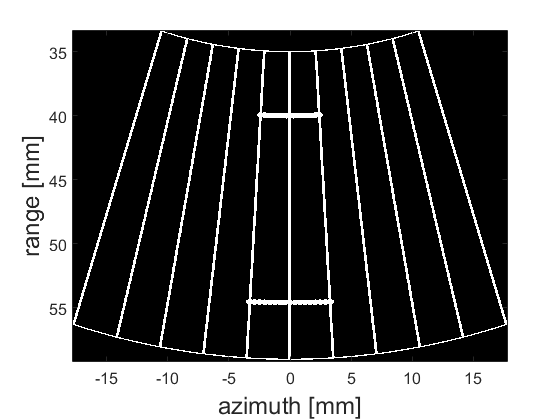
\includegraphics[width=\linewidth]{./images/results/1/illustration_scene.png}
    \caption{Illustration of whole scene}
    \label{fig:image_illustration}
    \end{subfigure}
    \quad
    \begin{subfigure}[t]{0.48\linewidth}
        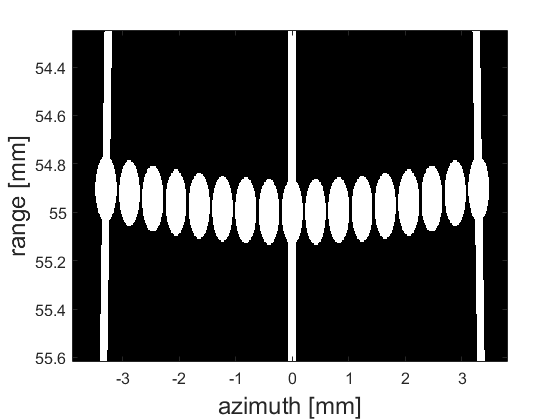
\includegraphics[width=\linewidth]{./images/results/1/zoom_55mm.png}
    \caption{Zoom around $55~$mm range}
    \label{fig:image_illustration_zoom}
    \end{subfigure}
	\caption{Illustration of imaged scene with 11 transmit beams and two scatterer points at $40~$mm and $55~$mm radius}
	\label{fig:frames_illustration}
\end{figure}

For each raw image, all four beamformers presented in Section \ref{sec:beamform_param} are used to produce a different beamformed image. As example of beamformed images, 2 of the 17 DAS beamformed frames are displayed in Figure \ref{fig:DAS_frame}, one with the scatterer points aligned with a beam trajectory ($0~$mm azimuth) and the other with the scatterer points in between two beams ($1.2~$mm and $1.65~$mm azimuth). Both scatterer points have lower apparent gain in Figure \ref{fig:DAS_frame2} than in Figure \ref{fig:DAS_frame1}.
Note that all the beamformed images displayed in this thesis are interpolated to yield smoother displays.
Although image interpolation is common practice before display, it is not applied to the raw data in order to avoid any potential artifact that could disturb the analysis.

\begin{figure}[ht]
    \centering
    \begin{subfigure}[t]{0.48\linewidth}
        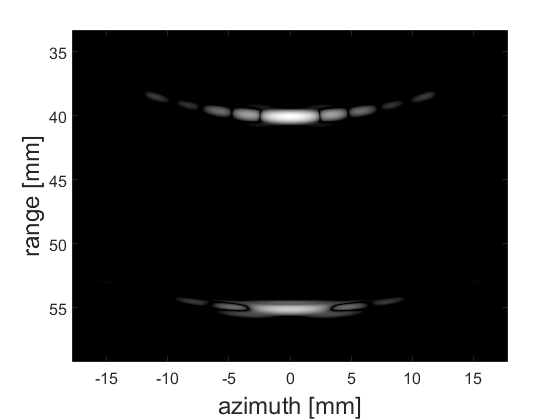
\includegraphics[width=\linewidth]{./images/results/1/DAS_frame1.png}
        \caption{Scatterer points at $0~$mm azimuth}
        \label{fig:DAS_frame1}
    \end{subfigure}
    \quad
    \begin{subfigure}[t]{0.48\linewidth}
        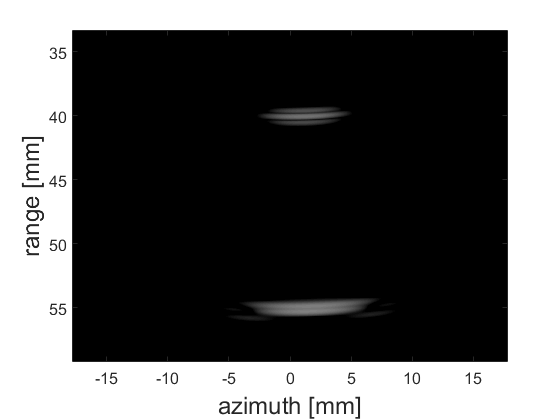
\includegraphics[width=\linewidth]{./images/results/1/DAS_frame2.png}
        \caption{Scatterer points at $1.2~$mm and $1.65~$mm azimuth}
        \label{fig:DAS_frame2}
    \end{subfigure}
	\caption{DAS beamformed image with 11 transmit beams and two scatterer points at $40~$mm and $55~$mm radius}
	\label{fig:DAS_frame}
\end{figure}

The variation in the backscattered signals gain is caused by scalloping loss, as explained in Section \ref{sec:beams_motion}. In this first experiment, for each beamformed image, the gain of the signals backscattered by each scatterer point is extracted and used for analysis.
The resulting gains are displayed in Figure \ref{fig:loss_vs_shift}.
Since the target of analysis is the difference in signal gain and not their absolute value, all gain values are normalized to that of the first frame.
Multiple observations can be made from these results. First of all the MV algorithm experiences much heavier scalloping loss than DAS in this example.
This is expected from the ability of the MV beamformer to form narrow receive beams compared to those of DAS.
This ability is the reason for the MV beamformer to be originally referred to as a high-resolution beamformer and is also the source of its increased sensitivity to angular undersampling compared to DAS.
Perhaps surprisingly, the IAA beamformers, also able to form narrow receive beams, are experiencing scalloping loss of lower or equal magnitude than DAS.
We do not want to draw conclusions based on a single experiment, but it seems at least in that example that the multibeam approach is effective in compensating for scalloping loss with angular undersampling.

As mentioned in Section \ref{sec:frames_motion}, in this thesis scalloping loss is considered invisible (and therefore negligible) if of magnitude lower or equal to 1 dB. 
A second observation is that, for all beamformers, the recorded gain of the scatterer points consistently appears to be maximized when they are aligned with a transmit beam and minimized when exactly in between two beams.
Given these results and the definition of \textit{scalloping loss} in Section \ref{sec:frames_motion}, the following experiments assume the maximum scalloping loss of a scatterer point to be its gain difference when aligned with a transmit beam and when exactly in between two beams. For example, the maximum scalloping loss of the MV beamformer for the scatterer point at $40~$mm radius is $43.2~$dB.

\begin{figure}[ht]
    \centering
    \begin{subfigure}[t]{\linewidth}
        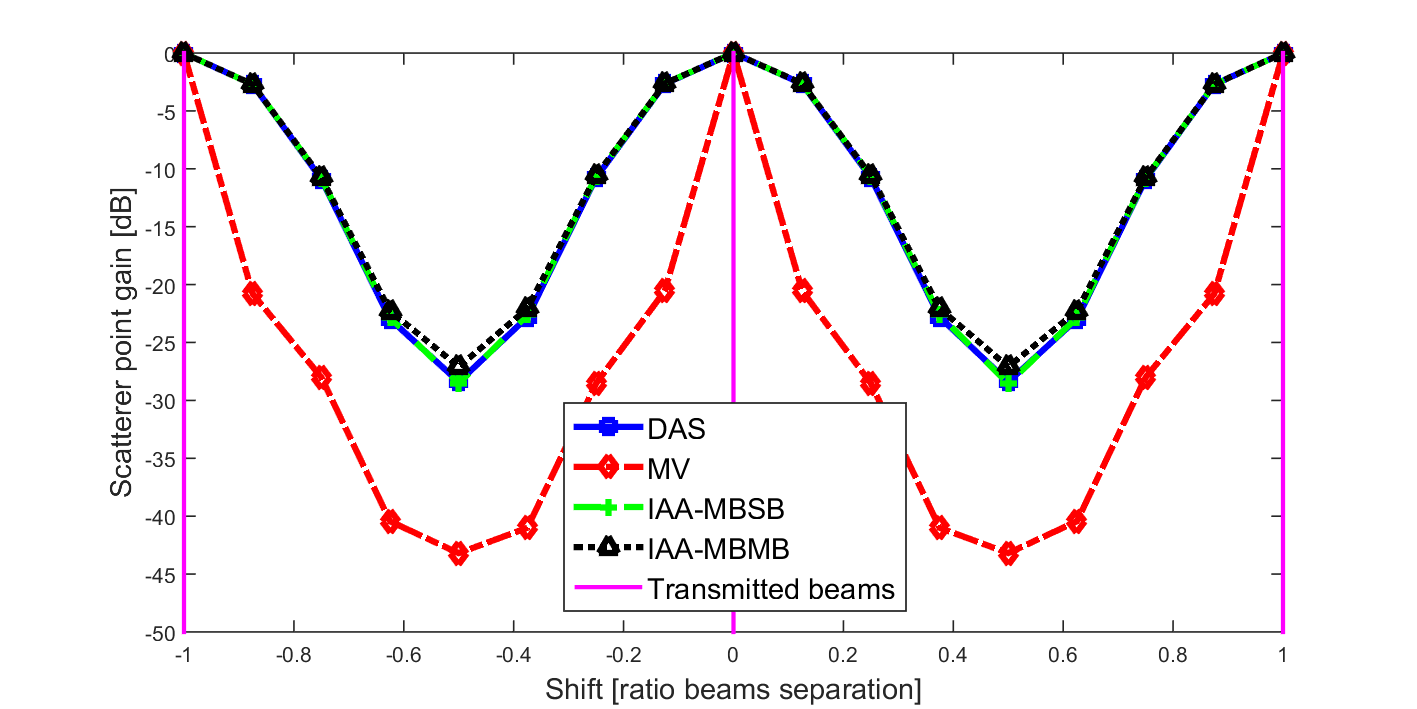
\includegraphics[width=\linewidth]{./images/results/1/loss_vs_shift_40mm.png}
        \caption{Scatterer point at $40~$mm radius}
    \end{subfigure}
    \quad
    \begin{subfigure}[t]{\linewidth}
        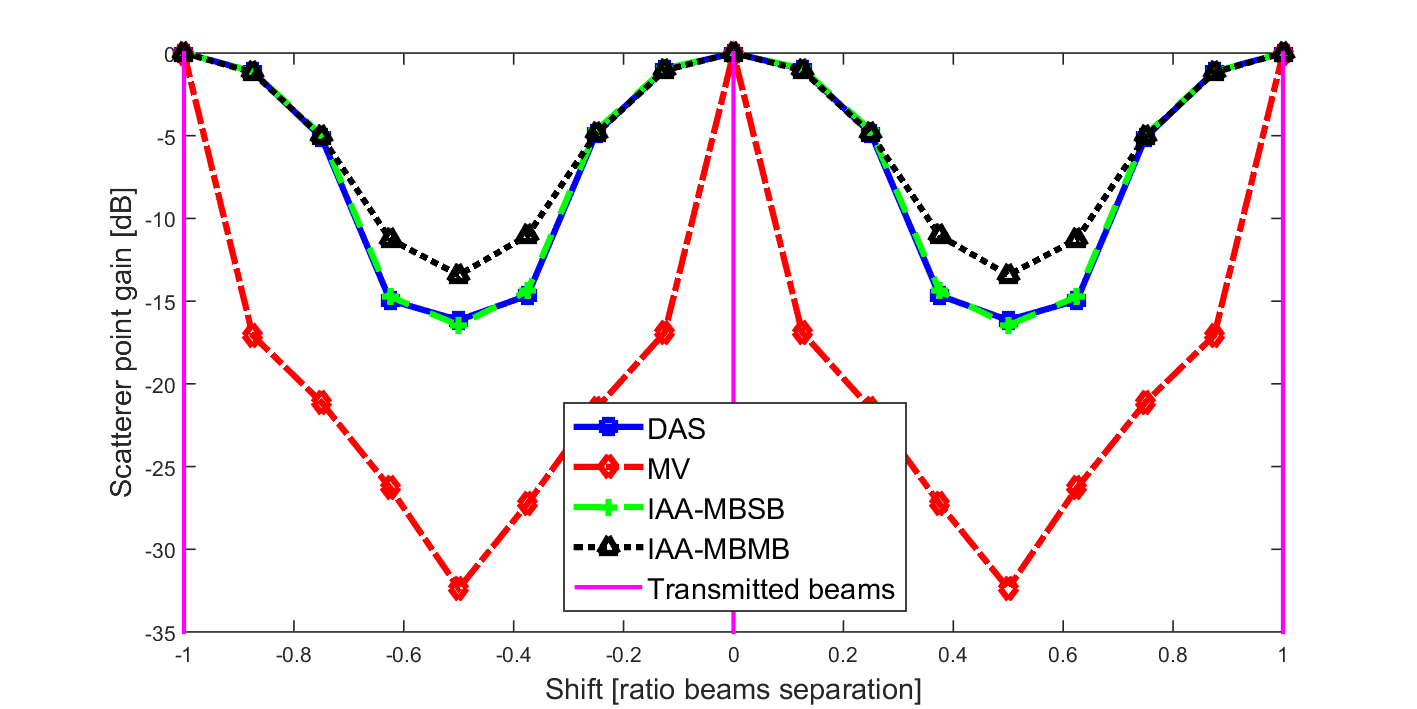
\includegraphics[width=\linewidth]{./images/results/1/loss_vs_shift_55mm.png}
        \caption{Scatterer point at $55~$mm radius}
    \end{subfigure}
	\caption{Normalized backscattered gain of scatterer point shifted 1/8th of the distance between beams per frame}
	\label{fig:loss_vs_shift}
\end{figure}


A final observation is that scalloping loss is more severe at $40~$mm radius than $55~$mm for all beamformers. In Section \ref{sec:frames_motion}, we emitted the hypothesis that scalloping loss can potentially be more severe at the array's focal distance than at any other radius.
In order to confirm that hypothesis, we set up an experiment similar to the previous one with a single scatterer point $s_1$ at various distances from the array, ranging from $36$ to $56~$mm radius.
For every given radius, we create two frames; one with $s_1$ aligned with the array's center transmit beam, at $0^\circ$ angle, and another frame with $s_1$ shifted along the same radius value so that it is placed exactly in between two beams.
For each beamformer and radius value, the scatterer point's recorded gain difference between the two frames defines its maximum scalloping loss.
The results of that experiment, displayed in Figure \ref{fig:loss_vs_range}, follow the hypothesis that the scalloping loss is most severe at the array's focal distance ($40~$mm radius).
The magnitude of scalloping loss experienced by the IAA approaches are again lower or roughly equal to that of DAS.
\begin{figure}[ht]
    \centering
    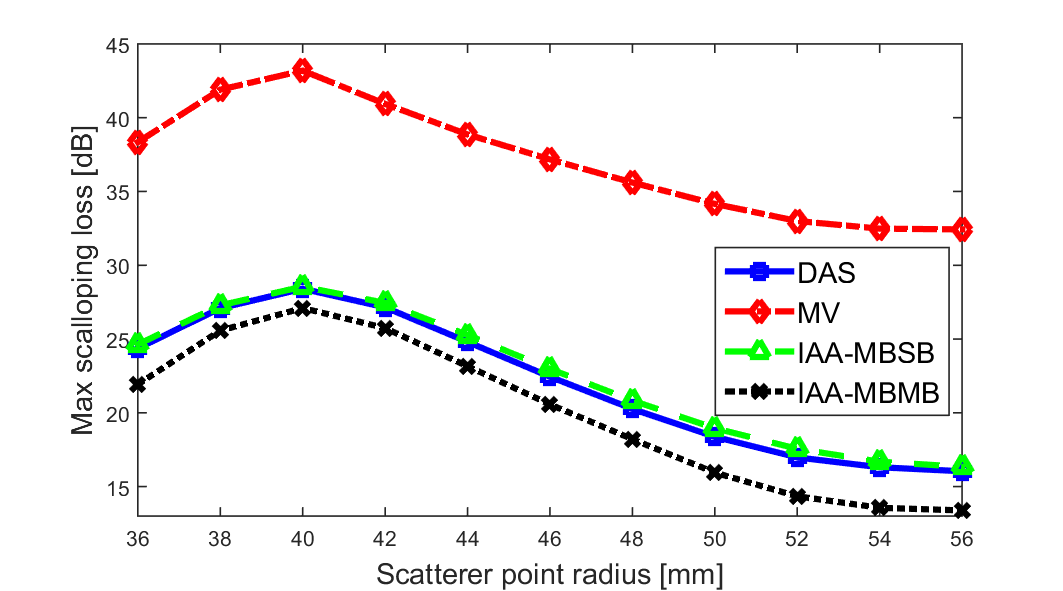
\includegraphics[width=\linewidth]{./images/results/1/loss_vs_range.png}
	\caption{Maximum scalloping loss of single point moving at constant radius}
	\label{fig:loss_vs_range}
\end{figure}

We are now able to define a worst case scenario regarding scalloping loss. The highest scalloping loss is expected to occur along the array's focus distance, assuming that the array's transmit focus line and receive focus line are the same.
Also assuming single-line acquisition (SLA), the highest scalloping loss for any given radius is expected to occur exactly in between two beams.
The highest scalloping loss magnitude is obtained in this thesis by simulating a scatterer point located at the array's focus distance ($40~$mm radius) and in between the array's center beam and its closest one towards the positive angle/azimuth values.
The following experiment recreates this worst case scenario with a noiseless medium.

We stated in Section \ref{sec:frames_motion} that there is an obvious dependence of the scalloping loss magnitude on the array's beam density and width.
We expect from \cite{Asen_shift_invariance} that scalloping loss can be reduced by increasing either the transmit and receive beam density and/or width.
Since the choice of beam width is a trade-off between angular sampling and image resolution, we prefer to focus on the choice of beam density in this section.
The transmit beam density gives a trade-off between angular sampling and image frame rate. We first focus on SLA beamforming.
For each transmit beam density $b_{tr}$, the maximum scalloping loss of each beamformer is recorded and displayed in Figure \ref{fig:loss_vs_beams}.

The DAS beamformer requires at least 65 beams to guarantee no visible scalloping loss in the imaged scene. Since the same algorithm is used for all beamformers for beams transmission, this number can be taken as basis for the required number of transmit beams $b_{tr}$. We think that the other beamformers can then achieve non-visible scalloping loss with $b_{tr} = 65$ by using parallel receive beamforming (PRB, Section \ref{sec:prb}). This can be done by creating multiple receive beams per transmit beam.
In this thesis, the beamformed images are obtained by sequentially transmit beams and, for each transmit beam, create a single receive beam aimed at the same focus point.
The perfect receive beam reconstruction is simulated by simply increasing the number of transmit beams so that $b_{tr} = b_{re}$.
Scalloping loss can obviously also be attenuated by simply increasing $b_{tr}$, but this results in an increased image acquisition time and therefore reduced frame rate. The transmit beam density is therefore always kept as low as possible.
The transmit beam density could be set even lower by increasing their width, but this would result in a resolution loss, as explained in Section \ref{sec:frames_motion}. 

As expected from Figures \ref{fig:loss_vs_shift} and \ref{fig:loss_vs_range}, the MV beamformer requires a much higher beam density than the other beamformers.
At the end of this section, we show an extension of Figure \ref{fig:loss_vs_range} for the MV beamformer with higher beam densities until invisible scalloping loss is achieved.
As expected from the previous experiments, the IAA-MB approaches are experiencing lower scalloping loss than DAS at low beams densities ($b_{re} < 35$ for IAA-MBSB and $b_{re} < 31$ for IAA-MBMB), but experience higher scalloping loss at higher beams densities. They require a higher beams density that DAS to avoid visible scalloping loss. This shows that the multibeam approach is good at attenuating major scalloping losses, by combining the information contained in several beams. However, since the IAA approaches are high-resolution beamformers, any remaining scalloping loss not corrected by the multibeam approach can be of higher magnitude than DAS due to the difference in their steered response mainlobe width.

\begin{figure}[ht]
    \centering
    \begin{subfigure}[t]{\linewidth}
        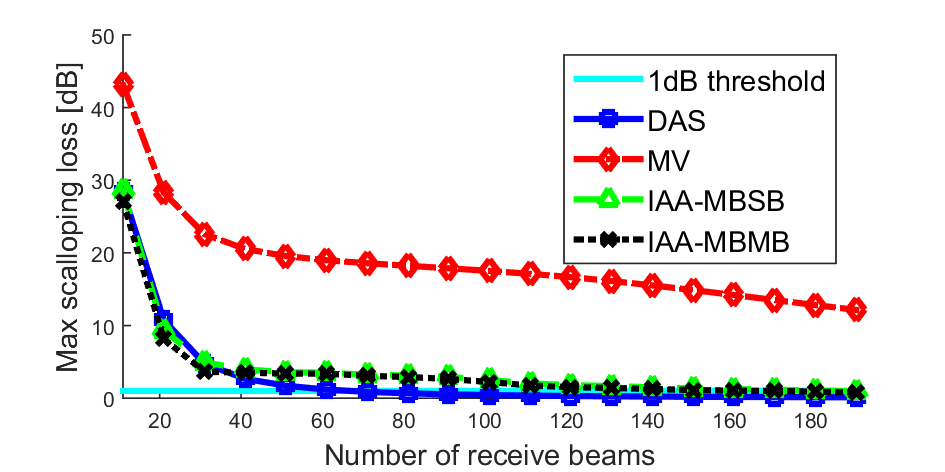
\includegraphics[width=\linewidth]{./images/results/1/loss_vs_beams.png}
        \caption{Whole plot}
    \end{subfigure}
    \quad
    \begin{subfigure}[t]{\linewidth}
        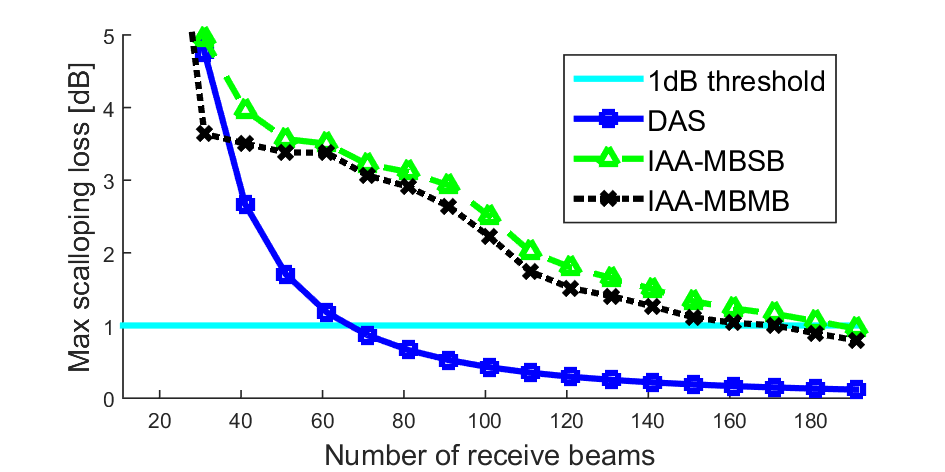
\includegraphics[width=\linewidth]{./images/results/1/loss_vs_beams_zoom.png}
        \caption{Plot focus on $[0, 5]~$dB range}
    \end{subfigure}
	\caption{Maximum scalloping loss of single scatterer point at $40~mm$ radius in noiseless medium}
	\label{fig:loss_vs_beams}
\end{figure}

The same experiment is then done on an imaged section containing speckle. Since speckle noise introduces randomness in the imaged medium, the same experiment is done with two different randomness generator seeds, $2$ and $42$.
Since a background with speckle noise is not smooth, different resolution cells can have different values, which means that a beamformer's maximum scalloping loss can not be estimated as done previously. The experiment displayed in Figure \ref{fig:loss_vs_shift} is reiterated here with a speckle background and displayed in Figure \ref{fig:loss_vs_shift_speckle}. The results show that the scatterer point minimum gain is not guaranteed to be exactly in between two beams anymore, due to the randomness of the background level. For that reason, for a given beam density $b_{tr}$, four frames are created with a single scatterer point shifted 1/4th of the angular distance between two beams per frame. Note that this does not guarantee to obtain the maximum possible scalloping loss, but it is considered in this thesis as good enough for the targeted accuracy. Those speckle simulations are indeed targeted to be used as examples of realistic divergences from the noiseless medium. Accurate analysis of speckle media would not only require a much higher number of frames per simulation, but also many more speckle background example in order to obtain meaningful statistical data. The scale of added computations and workload puts this out of the scope of this thesis.
\begin{figure}[ht]
    \centering
    \begin{subfigure}[t]{\linewidth}
        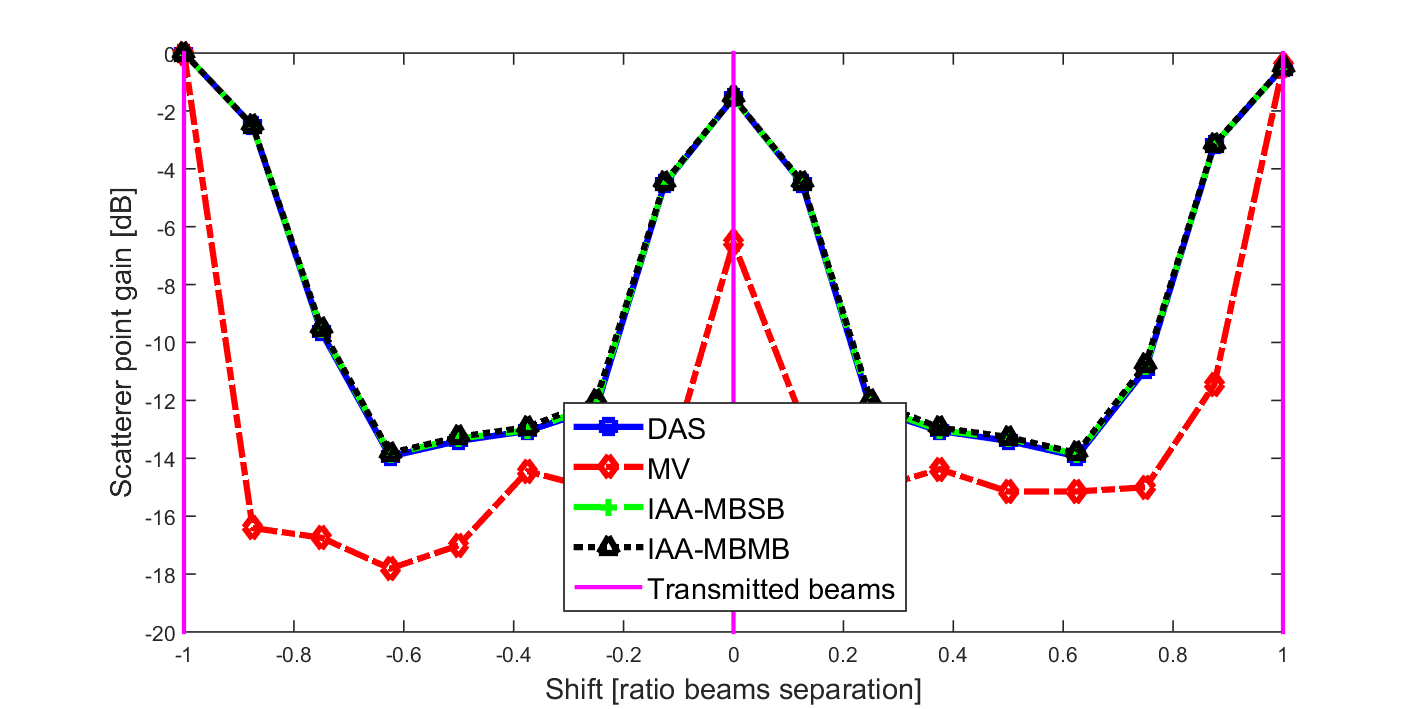
\includegraphics[width=\linewidth]{./images/results/1/loss_vs_shift_40mm_speckle.png}
        \caption{Scatterer point at $40~$mm radius}
    \end{subfigure}
    \quad
    \begin{subfigure}[t]{\linewidth}
        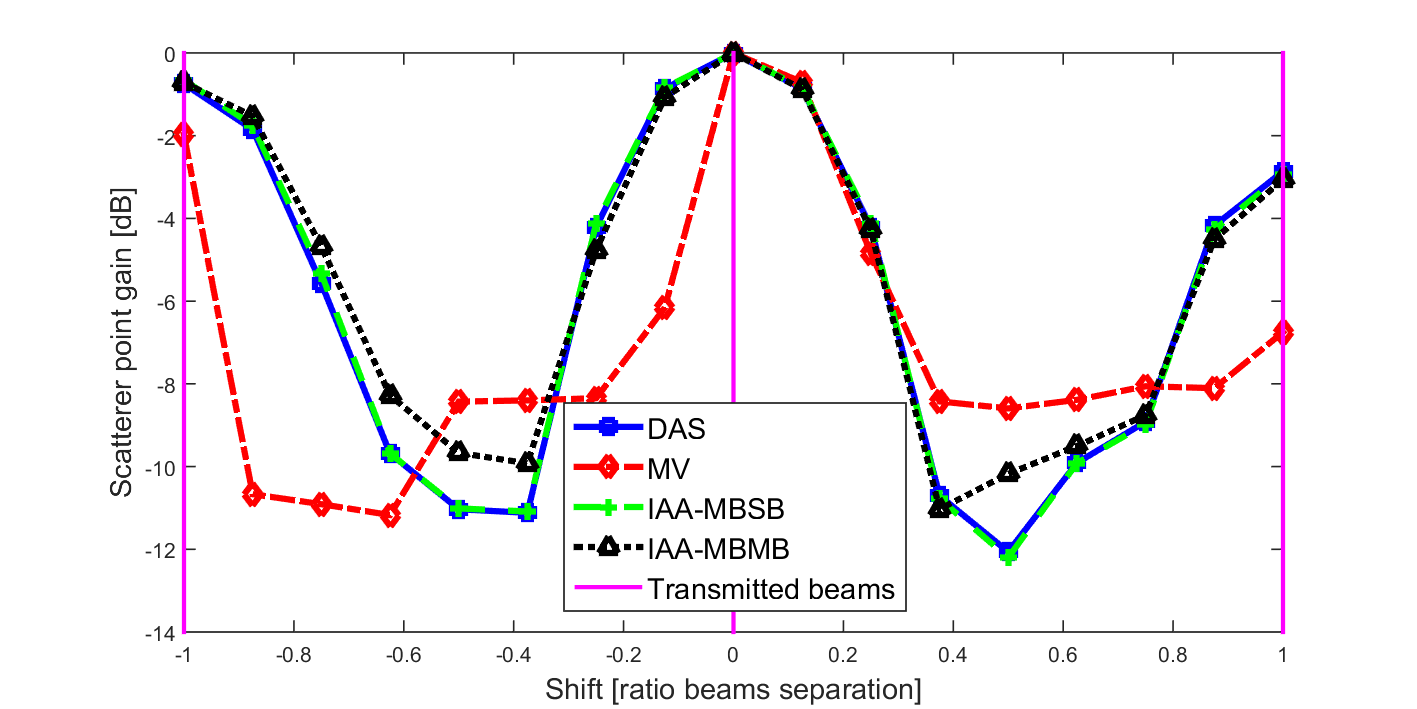
\includegraphics[width=\linewidth]{./images/results/1/loss_vs_shift_55mm_speckle.png}
        \caption{Scatterer point at $55~$mm radius}
    \end{subfigure}
	\caption{Normalized gain of scatterer point shifted 1/8th of distance between beams per frame in speckle background}
	\label{fig:loss_vs_shift_speckle}
\end{figure}

With the new approach to maximum scalloping loss estimation, the next experiment simulates a medium with speckle noise and a scatterer point at $40~$mm radius. The experiment is run with the two speckle backgrounds generated. The results are displayed in Figure \ref{fig:loss_vs_beams_speckle}.
As observed in the previous experiments, the MV algorithm experiences much heavier scalloping loss than the other beamformers. The IAA algorithm performs very well for an adaptive method, but some scalloping loss can still be visible for low beam densities. Another interesting observation is that the adaptive beamformers are more sensitive to the medium properties than the DAS one. They are sensitive to the presence of speckle noise and are consistently requiring fewer transmit beams to guarantee no visible scalloping loss.
This can easily be explained by the adaptive nature of the beamformers steered response. Adaptive beamformers can take advantage of directions towards which no or little energy is recorded and build steered responses with big sidelobes along those directions if it helps to build a higher and narrower mainlobe. The noiseless scenario can therefore produce globally narrower mainlobes, which results in an increase in their required density to avoid visible scalloping loss.
\begin{figure}[ht]
    \centering
    \begin{subfigure}[t]{\linewidth}
        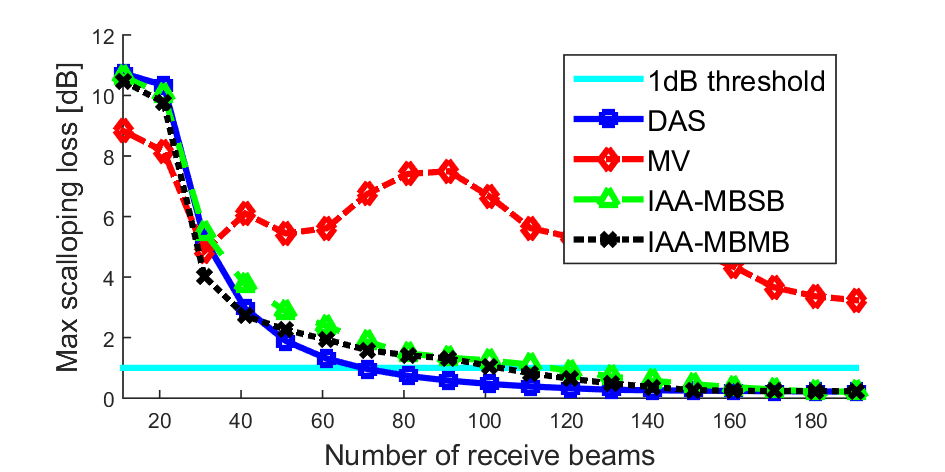
\includegraphics[width=\linewidth]{./images/results/1/loss_vs_beams_speckle2.png}
        \caption{Speckle seed 2}
    \end{subfigure}
    \quad
    \begin{subfigure}[t]{\linewidth}
        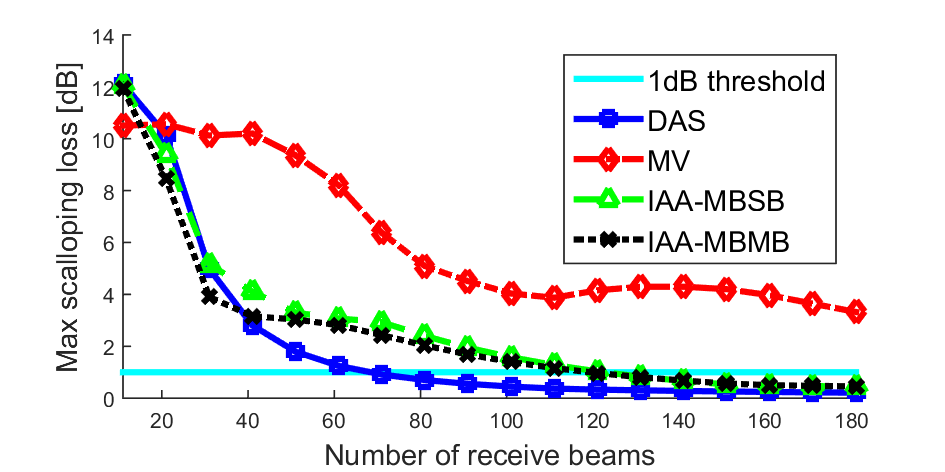
\includegraphics[width=\linewidth]{./images/results/1/loss_vs_beams_speckle42.png}
        \caption{Speckle seed 42}
    \end{subfigure}
	\caption{Maximum scalloping loss of single scatterer point at $40~$mm radius in speckle noise}
	\label{fig:loss_vs_beams_speckle}
\end{figure}

The required number of receive beams for each beamformer is summarized in Table \ref{table:num_beams}. The numbers for the MV beamformer are obtained from extending $b_{re}$ up to 981. An extension of Figures \ref{fig:loss_vs_beams} and \ref{fig:loss_vs_beams_speckle} for the MV beamformer is displayed in Figure \ref{fig:loss_vs_beams_ext}.
It is worth mentioning that 981 beams for 35 degrees coverage is well above typical beam densities and, even assuming that perfect PRB with $b_{re} > 15 \cdot b_{tr}$ is feasible, such a high number of receive beams may cause significant computational delays.
In practice, the required receive beam density may have to be reduced. This can be achieved to the cost of reduced resolution by for example increasing the diagonal load and/or by creating wider beams.

\begin{figure}[ht]
    \centering
        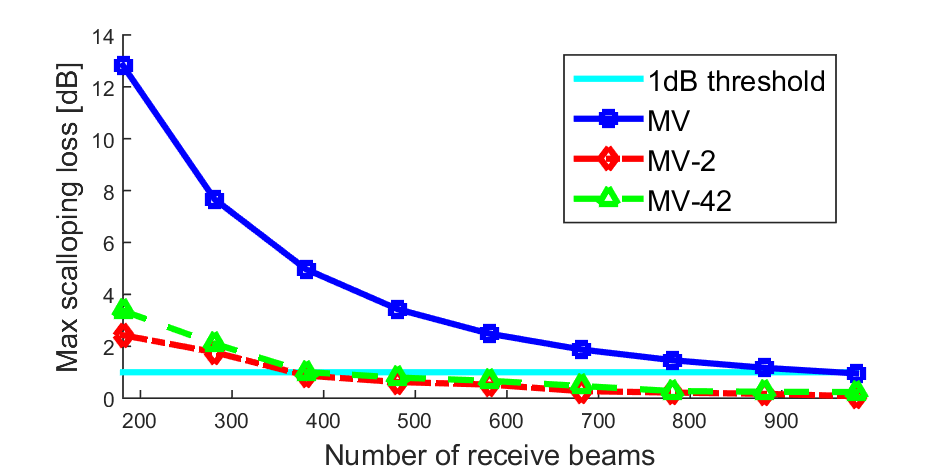
\includegraphics[width=\linewidth]{./images/results/1/loss_vs_beams_ext.png}
	\caption{MV Maximum scalloping loss of single scatterer point at $40~$mm radius in different media. MV is in noiseless medium, MV-2 and MV-42 in speckle noise (Seed 2, respectively 42)}
	\label{fig:loss_vs_beams_ext}
\end{figure}

\begin{table}[!ht]
\centering
\begin{tabular}{| c | c | c | c |}
  \hline
  Beamformer &   Without speckle   &   Speckle - seed 2 &   Speckle - seed 42 \\
  \hline
  DAS       &   65      &   71  &   71   \\
  MV        &   981     &   381  &   381 \\
  IAA-MBSB  &   191     &   101  &   123  \\
  IAA-MBMB  &   173     &   101 &   121  \\
  \hline
 \end{tabular}
\caption{Required number of beams for non-visible scalloping loss}
\label{table:num_beams}
\end{table}

As explained in Section \ref{sec:frames_motion}, the number of transmit beams has an impact on the beamformer's maximum frame rate. With $b_{tr} = 65$, the acquisition time of a single image can be obtained from Equation (\ref{eq:acquisition_time}): $t_{im} = 2 \cdot 0.15 \cdot 65 / 1500 = 13~$ms. In terms of frame rate (Equation (\ref{eq:frame_rate})), this results in a maximum of $f_{im} = 10^4 / (2 \cdot 65) = 76.9$ frames per second.
It is however important to mention that all images produced in this thesis are relatively small, only $2.5~$cm range and $35^\circ$ angular extent, and are produced with all beams focused at the same radius ($40~$mm). In many applications, bigger images are produced by creating beams with various focal radii. Many applications create images by sequentially transmitting and recording focused beams with a constant focal radius, such as done in this thesis, and repeat the sequence with a new focal radius. Each sequence is often referred to as a \textit{line of focus}. For images with multiple lines of focus, the maximum frame rate can be estimated to that of an image with single line of focus divided by the number of lines of focus.


\iffalse
As explained in Section \ref{sec:frames_motion}, the number of transmit beams has an impact on the beamformer's maximum frame rate. Table \ref{table:max_frame} combines the results of Table \ref{table:num_beams} and Equation \ref{eq:frame_rate}.

\textbf{What kind of frame rate is acceptable for real-time imaging?}

The MV beamformer requires too many transmit beams to both be used in real-time imaging and avoid visible scalloping loss. It is worth mentioning that 981 beams for 35 degrees coverage is well above typical beam densities and such a high number of beams would, on top of the physical acquisition delays, most probably cause significant computational delays. This remark is especially pertinent for the inversion of the covariance matrix estimate $\boldsymbol{\hat{R}}$.

The other beamformers appear to meet decent frame rate requirements for real-time imaging even in worst-case scenarios. However, it is important to mention that all images produced in this thesis are relatively small, only $2.5~$cm in range, and only are only produced with beams focused at the same radius ($40~$mm). In many applications, bigger images are produced by creating beams with various focal radius. Many applications create images by sequentially transmitting and recording focused beams with a constant focal radius, such as done in this thesis, and repeat the sequence with a new focal radius. Each sequence is often referred to as a \textit{line of focus}. For images with multiple lines of focus, the results of Table \ref{table:max_frame} can be extended to such images simply by dividing the frame rates by the number of lines of focus.
\textbf{What are typical number of focus lines when imaging organs?}

The frame rates of the IAA beamformers can therefore become insufficient for certain applications. Section \ref{sec:res_improvement} proposes improvement approaches and analysis their effects.

\begin{table}[!ht]
\centering
\begin{tabular}{| c | c | c | c |}
  \hline
  Beamformer &   Without speckle   &   Speckle - seed 2 &   Speckle - seed 42 \\
  \hline
  DAS       &   76.9     &   70.4 &   70.4  \\
  MV        &   5.1      &   13.1 &   13.1  \\
  IAA-MBSB  &   26.2     &   49.5 &   40.7  \\
  IAA-MBMB  &   28.9     &   49.5 &   41.3  \\
  \hline
 \end{tabular}
\caption{Maximum frame rate to guarantee no visible scalloping loss}
\label{table:max_frame}
\end{table}


Those figures show that the adaptive beamformers are very sensitive to the presence of speckle noise and are consistently requiring fewer transmit beams to guarantee no visible scalloping loss.
This can be explained by their adaptive nature, which allows them to adapt the shape of their steered response depending on the recorded wavefield. In this case, they can allow large steered response sidelobes in directions for which no or little energy is recorded in order to minimize its mainlobe width, thus increasing the resolution of the resulting image. The media containing speckle noise offer less freedom to the adaptive beamformers than noiseless ones, which then often results in larger mainlobes. The beams density requirements to avoid visible scalopping loss are therefore dropped
\fi